\label{sec:arch}



While the preceding section discussed world models as exogenous tools for policy training and evaluation—serving as simulation environments, reward models, or robust benchmarks—recent advances have shifted toward integrating world modeling directly into the policy architecture. This transition transforms the world model from an offline supervisor into an internal predictive core, enabling World Action Models (WAMs) to reason about world dynamics in real-time. 
We categorize these World Action Models architectures into two primary paradigms based on their structural flow and corresponding training regimes: (1) \textbf{Cascaded WAM} (\autoref{sec:cascaded_wam}) employs a sequential pipeline that first predicts the next state (e.g., in pixel, latent, or flow space) and subsequently derives the corresponding action. Due to this structural decoupling, they are characterized by a \textit{separated training} process where the world model and the action decoder are optimized as distinct modules; (2) \textbf{Joint WAM} (\autoref{sec:joint_wam}) unifies predictive state modeling and action generation within a single cohesive model, producing future states and actions simultaneously. In this paradigm, world modeling and action generation undergo \textit{joint training} under a unified objective, forcing the model to internalize the causal interdependencies between environmental dynamics and control signals.




Cascaded World-Action-Models implement the world-action mapping through a sequential two-stage pipeline: a world model first synthesizes a visual plan representing the anticipated future, after which a separate action model decodes executable robot commands from that plan. This decomposition offers a natural inductive bias — the world model need not reason about robot kinematics, while the action model need not solve long-horizon scene prediction — but it also introduces a coupling between the two stages that shapes every design decision within this family of approaches. Based on the type of intermediate planning carrier, Cascaded WAMs can be broadly categorized into two major classes: (1) \textbf{Explicit Planning} (\autoref{sec:cacaded_wam_explicit}) via pixel-space representations and (2) \textbf{Implicit Planning} (\autoref{sec:cacaded_wam_implicit}) via latent representations. \autoref{fig:cascaded_wam_taxonomy}  provides a schematic overview of these cascaded patterns.

\subsection{Cascaded World-Action-Model}

\label{sec:cascaded_wam}





\subsubsection{Explicit Planning via Pixel-Space Representations}

\label{sec:cacaded_wam_explicit}

The most direct realization of cascaded WAMs uses raw pixel frames as the intermediate representation between the two stages. Pixel-space plans are immediately interpretable and leverage the full representational capacity of large video generative models pretrained on internet-scale data, making them a natural starting point. Work in this space divides broadly by how actions are subsequently extracted from the synthesized video: through learned inverse dynamics, or through closed-form geometric computation.


\paragraph{Learned Action Extraction.}

\textbf{UniPi}~\cite{unipi} established the foundational two-stage blueprint: a text-conditioned spatiotemporal U-Net diffusion model synthesizes a task execution video, from which a convolutional inverse dynamics model (IDM) regresses actions between consecutive frame pairs. While demonstrating the viability of this closed loop, single-pass long-horizon generation was found to suffer from semantic drift and compounding errors. Subsequent work attacked this problem from complementary angles. \textbf{VLP}~\cite{du2023vlp} introduced semantic-level intervention by equipping the pipeline with a vision-language model (VLM) for hierarchical sub-action generation and tree-search-based value scoring, bounding error accumulation within each individual segment. \textbf{RoboEnvision}~\cite{yang2025roboenvision} instead adopted a non-autoregressive strategy, using VLM-decomposed subtask instructions to condition the generation of keyframes representing subtask terminal states, with full video subsequently synthesized by interpolation between those anchors.

Controllability and generation efficiency received focused attention in parallel. \textbf{ThisThat}~\cite{wang2024thisthat} addressed the fundamental ambiguity of language-only grounding in scenes containing multiple instances of the same object class by conditioning video generation jointly on deictic referring expressions (``this''/``that'') and paired gesture coordinates, transmitting manipulation intent without linguistic ambiguity. \textbf{Say, Dream, and Act}~\cite{gu2026saydreamact} pursued efficiency from a different direction, employing adversarial distillation to reduce denoising steps while introducing a frame-rate-agnostic video prediction mechanism that decouples trajectory planning from any fixed execution frequency, enabling unified prediction over variable-length horizons.

\begin{figure}
    \centering
    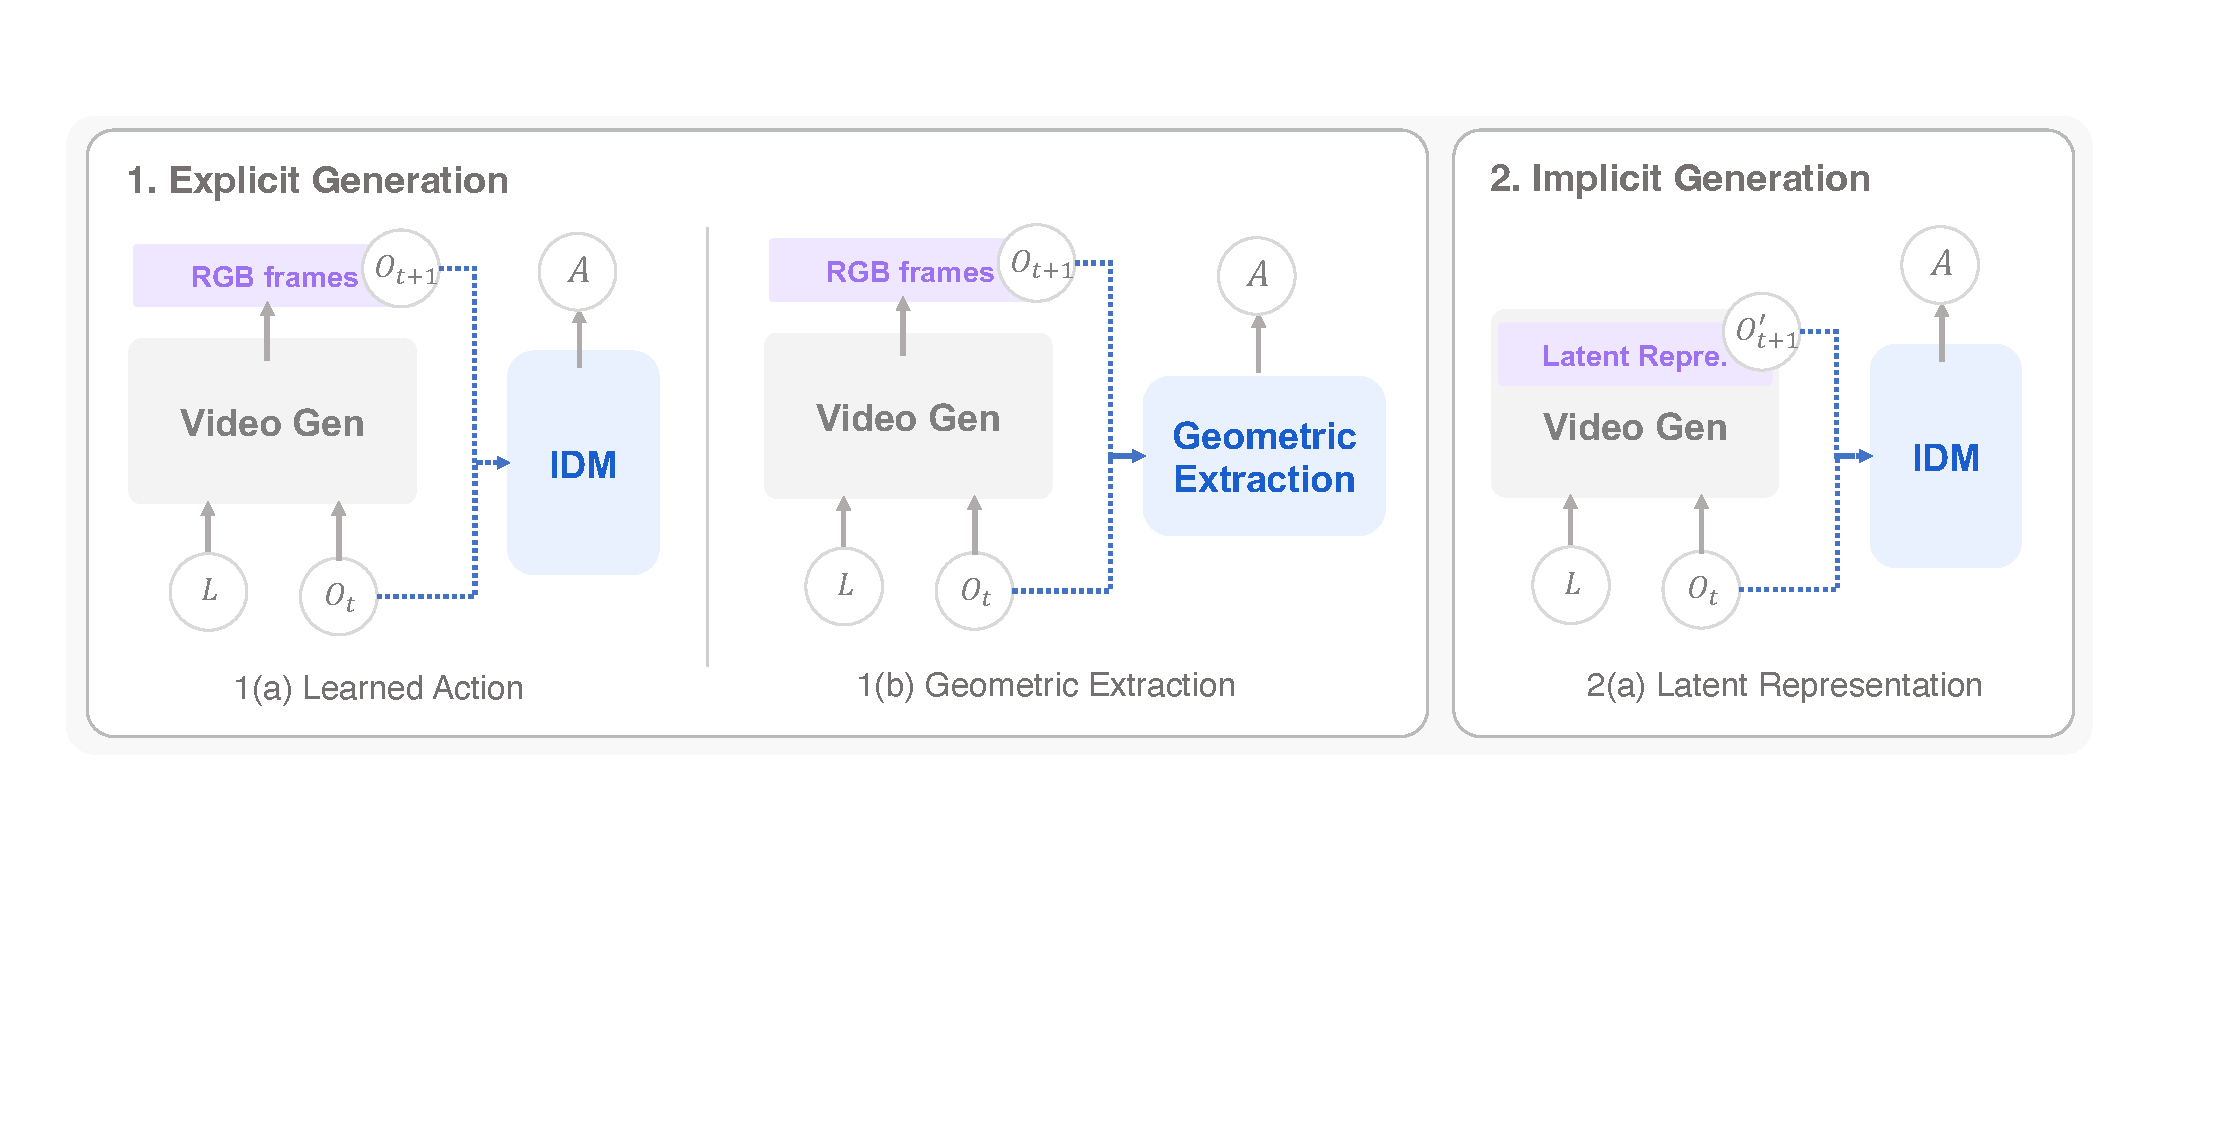
\includegraphics[width=1\linewidth]{pic/cascaded.pdf}
    \caption{Schematic comparison of cascaded WAM structures. \textbf{1(a) Learned Action}: a world model generates an explicit pixel-space future plan, which is mapped to actions by a learned inverse-dynamics or action model. \textbf{1(b) Geometric Extraction}: the explicit visual plan is converted into actions or trajectories through geometric extraction. \textbf{2(a) Latent Representation}: the intermediate planning carrier is a latent future representation rather than future RGB frames, and the downstream action model decodes executable commands from it.}
    \label{fig:cascaded_wam_taxonomy}
\end{figure}

The spatial expressiveness of the planning representation has also been extended beyond standard RGB video. \textbf{TesserAct}~\cite{TesserAct1} augments the video prediction target with depth and surface normal channels, introducing explicit geometric constraints into the planning carrier and providing richer cues for downstream action extraction. \textbf{MVISTA-4D}~\cite{wang2026mvista4d} replaces the conventional IDM entirely with a two-step mechanism consisting of trajectory-level latent optimization followed by residual IDM refinement, alleviating the ill-posed nature of per-step action extraction.

Extending the approach across embodiment types and data sources has driven a further line of work. \textbf{Vidar}~\cite{vidar} builds on a diffusion-based video foundation model to translate human manipulation videos into robot execution videos, simultaneously addressing unified bimanual robot modeling by encoding robot type, camera layout, task instructions, and scene context as global generation conditions with masked prediction to focus on interaction-critical regions. \textbf{Gen2Act}~\cite{bharadhwaj2024gen2act} pushes further toward embodiment-agnostic operation by calling a pretrained \textbf{VideoPoet}~\cite{VideoPoet} model zero-shot to generate human manipulation video without any fine-tuning, and replacing hard-coded geometric extraction rules with a closed-loop neural policy that uses point tracking as an auxiliary loss to implicitly encode motion information.
\textbf{Veo-Act}~\cite{zhang2026veoact} addresses the precision gap of foundation video models in contact-rich phases via a gating mechanism: a multi-head IDM extracts actions from Veo-3-generated video for coarse navigation, and an online interaction detector hands control over to a reactive VLA policy once imminent contact is detected.

Rather than extracting actions via a specific IDM, several works replace it with alternative decoders. \textbf{VAG}~\cite{lang2026vag} adopts a 1D U-Net as the action decoder: the video diffusion branch completes the full denoising process to pixel space, and intermediate features from the video U-Net condition a separate action U-Net. \textbf{$\pi_{0.7}$}~\cite{pi0.7} replaces the second stage IDM with a pretrained VLA. A BAGEL-based world model \cite{bagel} generates multi-view subgoal images of the desired near-future state, which are injected directly into the VLA's context window alongside language and episode metadata; the VLA's flow-matching action expert then produces action chunks conditioned on this imagined future. This shifts the burden of generalization from inverse dynamics learning to the VLA's pretrained in-context understanding, enabling strong out-of-the-box and zero-shot cross-embodiment performance without task-specific fine-tuning. 



\paragraph{Geometric Action Extraction.}
A parallel line of work replaces the learned IDM with geometric computation over structured intermediate representations, converting the action extraction problem from an inverse dynamics learning problem into an analytically tractable geometric one. This family divides by whether motion is represented as optical flow or as tracked object poses.

Optical flow as an intermediate representation was introduced by \textbf{AVDC}~\cite{ko2024avdc}, which separates video synthesis from action extraction entirely: a text-conditioned diffusion model generates full pixel-level video, from which dense optical flow is computed and SE(3) transformations are analytically derived, requiring no action annotations during training.

\newcommand{\yes}{$\checkmark$}
\newcommand{\no}{$\times$}



\begin{table}[!t] 
\centering
\scriptsize
\setlength{\tabcolsep}{3.5pt}
\renewcommand{\arraystretch}{1.08}
\caption{Comparison of Cascaded World-Action-Model (WAM) methods. \textbf{Act.\ Label}: whether action annotations are required. \textbf{Zero-shot}: no task-specific training/fine-tuning needed. Sim = simulation benchmark; Real = physical robot.}
\label{tab:cascaded_wam}

\begin{adjustbox}{width=\linewidth}
\begin{threeparttable}
\begin{tabular}{
  l
  >{\RaggedRight\arraybackslash}p{2.20cm}
  >{\RaggedRight\arraybackslash}p{3.50cm}
  >{\RaggedRight\arraybackslash}p{3.60cm}
  l
  l
  >{\RaggedRight\arraybackslash}p{5.80cm}
}
\toprule
\textbf{Method} &
\textbf{Interm.\ Repr.} &
\textbf{Stage-1 Backbone} &
\textbf{Stage-2 Model} &
\makecell{\textbf{Act.}\\\textbf{Label}} &
\makecell{\textbf{Zero-}\\\textbf{shot}} &
\textbf{Evaluation} \\
\midrule

% -------------------------------------------------------
\rowcolor{gray!12}
\multicolumn{7}{l}{\textbf{Pixel-space Representations --- Learned Action Extraction}} \\
\midrule
UniPi \cite{unipi}
  & Pixel RGB
  & Video U-Net
  & Lightweight IDM (CNN\,+\,MLP)
  & \yes & \no
  & Sim: PDSketch block manip., CLIPort \newline Real: WidowX \\
VLP \cite{du2023vlp}
  & Pixel RGB
  & Video U-Net\,+\,PaLM-E 12B
  & LAVA
  & \yes & \no
  & Sim: Language Table \newline Real: Language Table robot, 7-DoF mobile arm, 14-DoF ALOHA bimanual \\
RoboEnvision \cite{yang2025roboenvision}
  & Pixel RGB
  & OpenSora (DiT)
  & OpenSora DiT
  & \yes & \no
  & Sim: LanguageTable, LHMM (custom) \newline Real: - \\
This\&That \cite{wang2024thisthat}
  & Pixel RGB
  & U-Net
  & Custom closed-loop neural policy
  & \yes & \no
  & Sim: IsaacGym \newline Real: - \\
Say, Dream \& Act \cite{gu2026saydreamact}
  & Pixel RGB
  & COSMOS-PREDICT2
  & Transformer (ACT)\,+\,Qwen2.5
  & \yes & \no
  & Sim: LIBERO \newline Real: Franka 7-DoF arm \\
TesserAct \cite{TesserAct1}
  & Pixel RGB-DN
  & CogVideoX (DiT)
  & PointNet++, MLP
  & \yes & \no
  & Sim: RLBench \newline Real: - \\
MVISTA-4D \cite{wang2026mvista4d}
  & Pixel RGB-D
  & WAN2.2 TI2V
  & PointNet
  & \yes & \no
  & Sim: RLBench, RoboTwin2 \newline Real: AgileX Piper \\
Vidar \cite{vidar}
  & Pixel RGB
  & Wan2.2 (sim)\,/\,Vidu~2.0 (real)
  & Masked IDM (MIDM)
  & \yes & \no
  & Sim: RoboTwin 2.0 \newline Real: Aloha \\
Gen2Act \cite{bharadhwaj2024gen2act}
  & Pixel RGB
  & VideoPoet
  & Custom closed-loop neural policy
  & \yes & \no
  & Sim: - \newline Real: Mobile manipulation robot \\
Veo-Act \cite{zhang2026veoact}
  & Pixel RGB
  & Veo-3
  & Multi-head IDM + VLA ($\pi_{0.5}$)
  & \yes & \no
  & Sim: IsaacLab \newline Real: 7-DoF arm\,+\,12-DoF dexterous hand \\
VAG \cite{lang2026vag}
  & Pixel RGB
  & Cosmos-Predict2
  & 1D U-Net
  & \yes & \no
  & Sim: LIBERO \newline Real: AgiBot G1, AgileX Cobot Magic \\
$\pi_{0.7}$ \cite{pi0.7}
  & Pixel RGB 
  & BAGEL 
  & VLA
  & \yes & \no
  & Sim: - \newline Real: Mobile manipulators, Static bimanual, UR5e \\
\midrule
% -------------------------------------------------------
\rowcolor{gray!12}
\multicolumn{7}{l}{\textbf{Pixel-space Representations --- Geometric Extraction}} \\
\midrule
AVDC \cite{ko2024avdc}
  & Pixel RGB $\to$ optical flow
  & U-Net
  & Off-the-shelf geometric pipeline (learning-free)
  & \no & \no
  & Sim: Meta-World, iTHOR \newline Real: Franka Emika Panda \\
Im2Flow2Act \cite{xu2024im2flow2act}
  & Optical flow
  & AnimateDiff\,+\,Stable Diffusion (latent)
  & Flow-conditioned IL policy
  & \yes & \no
  & Sim: Custom tasks \newline Real: UR5e \\
3DFlowAction \cite{zhi2025threedflowaction}
  & 3-D optical flow
  & AnimateDiff\,+\,Stable Diffusion
  & Flow-constrained optimization policy
  & \no & \no
  & Sim: Custom tasks \newline Real: Franka, XTrainer \\
NovaFlow \cite{li2025novaflow}
  & Optical flow
  & Wan~2.1\,+\,off-the-shelf modules
  & Flow-based executor
  & \no & \yes
  & Sim: - \newline Real: Franka Emika Panda, Boston Dynamics Spot \\
Dream2Flow \cite{dharmarajan2025dream2flow}
  & Optical flow
  & Off-the-shelf I2V model
  & CoTrackerV3\,+\,trajectory opt.\,/\,RL
  & \no & \yes
  & Sim: OmniGibson, RoboSuite \newline Real: Franka arm, Spot, GR1 humanoid \\
% \midrule
% -------------------------------------------------------
% \rowcolor{gray!12}
% \multicolumn{7}{l}{\textbf{Pixel-space Representations --- Geometric Extraction (Pose Tracking)}} \\
Dreamitate \cite{liang2024dreamitate}
  & Pixel RGB
  & U-Net
  & MegaPose
  & \no & \no
  & Sim: - \newline Real: UFACTORY xArm~7, UR5 \\
4DGen \cite{liu2025fourdgen}
  & Pixel RGB-D\,+\,4-D point maps
  & U-Net
  & FoundationPose\,+\,SAM2
  & \no & \no
  & Sim: LBM \newline Real: Dual Franka Panda \\
RIGVid \cite{patel2025rigvid}
  & Pixel RGB
  & Kling v1.6
  & GPT-4o, depth estimator,\allowbreak FoundationPose,\allowbreak Grounding DINO\,+\,SAM-2,\allowbreak AnyGrasp
  & \no & \yes
  & Sim: - \newline Real: XArm7, Aloha \\
LV-P \cite{chen2025lvp}
  & Pixel RGB
  & WAN~2.1 I2V 14B
  & HaMeR, MegaSAM,\allowbreak Dex-Retargeting, cuRobo
  & \no & \yes
  & Sim: - \newline Real: Franka Emika\,+\,parallel gripper, Unitree G1\,+\,Inspire dexterous hand \\
\midrule

% -------------------------------------------------------
\rowcolor{gray!12}
\multicolumn{7}{l}{\textbf{Implicit Planning via Latent Representations}} \\
\midrule
Video Policy \cite{liang2025videopolicy}
  & Latent features
  & U-Net
  & Action U-Net
  & \yes & \no
  & Sim: RoboCasa, Libero10 \newline Real: Unspecified \\
ARDuP \cite{huang2024ardup}
  & Latent video frames\,+\,active-region encoding
  & U-Net
  & Lightweight CNN
  & \yes & \no
  & Sim: CLIPort \newline Real: WidowX \\
mimic-video \cite{pai2025mimicvideo}
  & Latent video
  & Cosmos-Predict2
  & Action Decoder DiT
  & \yes & \no
  & Sim: SIMPLER-Bridge, LIBERO \newline Real: Dual Franka Emika Panda\,+\,16-DoF dexterous hands \\
VPP \cite{hu2024vpp}
  & Latent video
  & Stable Video Diffusion
  & VideoFormer\,+\,DiT Diffusion Policy
  & \yes & \no
  & Sim: CALVIN, MetaWorld \newline Real: Franka Panda, Xarm\,+\,12-DoF Xhand \\
VILP \cite{xu2025vilp}
  & Latent video
  & U-Net\,+\,3-D convolution
  & Two CNN encoders\,+\,MLP head
  & \yes & \no
  & Sim: Custom tasks \newline Real: Franka Panda \\
LAPA \cite{LAPA}
  & Discrete latent action tokens
  & C-ViViT tokenizer
  & LWM-Chat-1M
  & \yes & \no
  & Sim: Language Table, SIMPLER \newline Real: 7-DoF Franka Emika Panda \\
villa-X \cite{chen2025villax}
  & Discrete latent action tokens
  & Spatial-Temporal Transformer \,+\,ViT \,+\,proprio FDM
  & PaliGemma VLM
  & \yes & \no
  & Sim: SIMPLER, LIBERO \newline Real: gripper manip., dexterous hand manip. \\
S-VAM \cite{yan2026svam}
  & Latent features
  & Stable Video Diffusion
  & Uni-Perceiver
  & \yes & \no
  & Sim: CALVIN, MetaWorld \newline Real: AgileX Cobot dual-arm \\
OmniVTA \cite{zheng2026omnivta}
  & Latent tactile features
  & Two-stream DiT
  & Diffusion Policy\,+\,MLP controller
  & \yes & \no
  & Sim: - \newline Real: 7-DoF xArm\,+\,tactile sensors \\
MWM \cite{lou2026mwm}
 & Latent features
 & DiT
 & Diffusion Policy
 & \yes & \no
 & Sim: LIBERO, RLBench \newline Real: Franka  \\
\bottomrule
\end{tabular}
\end{threeparttable}
\end{adjustbox}
\end{table}
\textbf{Im2Flow2Act}~\cite{xu2024im2flow2act} relocates flow estimation to latent space, using an \textbf{AnimateDiff}~\cite{guo2024animatediff}-based flow generation network to bypass pixel-level video synthesis altogether; a separately trained flow-conditioned policy then maps the flow field directly to actions, trading pixel-level appearance information for computational efficiency. \textbf{3DFlowAction}~\cite{zhi2025threedflowaction} lifts this representation from two dimensions to three, using video diffusion to generate dense three-dimensional flow fields that capture rotational and depth-displacement motion components inaccessible to planar flow. \textbf{NovaFlow}~\cite{li2025novaflow} and \textbf{Dream2Flow}~\cite{dharmarajan2025dream2flow} push the paradigm toward zero-training operation, using pretrained video generation models directly and deriving three-dimensional object-level flow via depth estimation and point tracking before converting to robot commands without demonstration data or additional training.

Pose tracking constitutes the second geometric extraction route. \textbf{Dreamitate}~\cite{liang2024dreamitate} uses a tool as the linking proxy between human and robot action: a stereo video diffusion model fine-tuned on human tool-use demonstrations generates task execution video conditioned on stereo scene images, from which \textbf{MegaPose}~\cite{labbe2022megapose} tracks the tool's 6-DoF pose frame-by-frame; stereo geometry constrains depth estimation, and inverse kinematics maps the resulting trajectory to joint commands, making action extraction entirely independent of robot morphology. \textbf{4DGen}~\cite{liu2025fourdgen} extends this to multi-view consistent generation, jointly predicting RGB video and three-dimensional point map sequences from two-view RGB-D conditioning using an SVD backbone. \textbf{RIGVid}~\cite{patel2025rigvid} applies \textbf{FoundationPose}~\cite{wen2024foundationpose} to track the manipulated object rather than the tool, replaces inverse kinematics with trajectory retargeting, and substitutes human demonstration video with zero-shot diffusion-generated video filtered for quality by a VLM. \textbf{LVP}~\cite{chen2025lvp} reconstructs three-dimensional hand poses from generated human manipulation video and maps them to end-effector trajectories through kinematic mapping, while adopting Diffusion Forcing — partitioning video into low-noise historical and high-noise future segments with causal masking — to improve temporal coherence in generation.

\subsubsection{Implicit Planning via Latent Representations}

\label{sec:cacaded_wam_implicit}

The computational overhead of pixel-level video synthesis constitutes the primary bottleneck against real-time deployment. The implicit planning path is motivated by the observation that intermediate latent representations formed during diffusion already encode the dynamical information required for planning; decoding back to pixel space is therefore unnecessary. The planning carrier is replaced by latent feature sequences that remain in the compressed representation space throughout.

\textbf{VPP}~\cite{hu2024vpp} demonstrated this trade-off directly: a pretrained VAE encodes observation frames, a diffusion model performs single-step prediction of future latent sequences, and a lightweight policy network conditions on these latents to produce actions, achieving planning inference speeds compatible with real-time control for the first time in this framework. \textbf{VILP}~\cite{xu2025vilp} introduced multi-view latent planning within the same paradigm, generating complete latent video sequences from two simultaneous viewpoints and recovering actions with a separately trained state policy network.
\textbf{S-VAM}~\cite{yan2026svam} directly addresses the generation quality cost incurred by VPP's single-step inference, using self-distillation to bridge the gap between efficiency and fidelity: during training, a frozen multi-step SVD backbone provides structured teacher representations that supervise lightweight spatio-temporal decouplers, condensing iterative generation into a single forward pass. At inference, one-step features are aggregated via a QFormer-style perceiver and condition a DiT-based diffusion policy, recovering high-quality planning at real-time control frequencies.


\textbf{Video Policy}~\cite{liang2025videopolicy}, while using explicit pixel video in its first stage, pioneered a key implicit extraction technique: after fine-tuning SVD for video prediction, all video U-Net weights are frozen and a separate action U-Net is trained to generate action sequences conditioned on intermediate features from the video decoder, establishing feature-level conditioning as an alternative to pixel or flow inputs. \textbf{ARDuP}~\cite{huang2024ardup} derives pseudo-supervision from \textbf{Co-Tracker}~\cite{karaev2023cotracker} dense motion point tracking and \textbf{SAM}~\cite{kirillov2023sam}-generated interaction region masks during training, using the resulting active-region proposals as conditions injected into a video diffusion model to concentrate generation on task-relevant areas. \textbf{mimic-video}~\cite{pai2025mimicvideo} advances generation efficiency through flow matching in place of DDPM and a partial denoising strategy that extracts features at an intermediate ODE integration checkpoint, bypassing the full generation path. \textbf{MWM}~\cite{lou2026mwm} replaces RGB prediction with future semantic mask latents, caching the hidden states from its frozen mask-forecasting backbone to condition an action diffusion head. This geometric information bottleneck effectively filters out photometric nuisances, yielding highly robust control under severe visual shifts.

\textbf{OmniVTA}~\cite{zheng2026omnivta} extends implicit latent planning to the visuo-tactile domain. A two-stream diffusion transformer jointly generates future visual and tactile latents, and a downstream fusion policy consumes the predicted tactile latents via a differential encoder that captures discrepancies between predicted and current contact states, enabling robust generalization to unseen objects in contact-rich manipulation.

\textbf{LAPA}~\cite{LAPA} proposes an unsupervised latent action pretraining framework: a \textbf{VQ-VAE}~\cite{oord2017vqvae}-based latent action model learns ``state-latent action'' priors from unlabeled videos in a self-supervised manner, requiring only a small amount of real action annotations during downstream fine-tuning to map to actual joint actions, significantly reducing annotation demands. \textbf{villa-X}~\cite{chen2025villax} advances latent action modeling in two key aspects. First, a proprioceptive Forward Dynamics Model (proprio-FDM) is incorporated to ground latent actions in physical dynamics through joint optimization of visual reconstruction and proprioceptive prediction losses. Second, a joint diffusion framework comprising a latent action expert and a robot action expert is proposed, whereby latent actions explicitly condition low-level action generation for more structured knowledge transfer.





\subsection{Joint World-Action-Model}

\label{sec:joint_wam}
Joint World-Action Models denote a family of architectures in which future world states and actions are predicted within a single unified model, with both world modeling and action generation serving as joint supervision targets during training \cite{PAD,UWM,UVA,PhysGen,FLARE,FRAPPE,CosmosPolicy,Motus,Act2Goal,DUST,DiT4DiT,CoVAR}. 
The central design question for joint architectures is therefore how world state and action generation are coupled within the shared predictive system. Under this unified definition, existing joint world-action models can be further organized into two broad generation routes according to the substrate on which world--action prediction is realized：(1) \textbf{Autoregressive Generation} (\autoref{sec:joint_discerte}), in which future world variables and action variables are serialized into token space and modeled through autoregressive prediction; (2) \textbf{Diffusion-based Non-Autoregressive Generation} (\autoref{sec:joint_continuous}), in which future observations, latent world states, or action trajectories are generated through diffusion- or flow-based generative processes, enabling the joint refinement of both modalities within a continuous latent space or through parallel denoising streams.



\subsubsection{Joint Prediction via Autoregressive Generation}
% \subsubsection{Joint Prediction via Discrete Tokenization}
\label{sec:joint_discerte}

\textbf{Autoregressive Generation} denotes the branch of joint world-action models that rely on causal, left-to-right sequential decoding to parameterize both future states and control signals \cite{GR1, grmg, GR2, CoTVLA, WorldVLA, rynnvla2, VLA-JEPA}. In these architectures, heterogeneous variables are serialized into a unified temporal sequence where the joint distribution of world and action is factorized sequentially. This fundamental generative mechanism ensures that earlier predictions causally condition subsequent steps within a given generation window.

However, while this shared reliance on \textbf{causal sequence modeling} unifies these architectures, casting control and video generation into a strict left-to-right prediction problem introduces profound architectural tensions. The primary challenge lies in mitigating catastrophic error propagation—where early visual hallucinations cascade into subsequent action failures—while balancing the inherent computational bottleneck of sequential decoding against the low-latency demands of real-time robotic execution.



Within this branch, we organize the literature by tracing the evolution of their underlying target representations and output interfaces. We identify three distinct representational paradigms: (1) \textbf{Explicit Decoupled Representation}, where modalities maintain heterogeneous formats and are decoded through structurally separate output heads; (2) \textbf{Unified Discrete Representations}, where modalities are fully quantized into a homogeneous token space and governed by a shared prediction head; and (3) \textbf{Predictive Latent Representations}, which abandon explicit token generation in favor of autoregressing over abstract, continuous latent spaces.





\begin{table}[t]
\centering
\scriptsize
\setlength{\tabcolsep}{3.5pt}
\renewcommand{\arraystretch}{1.08}
\caption{Taxonomy-oriented summary of \textbf{Autoregressive Generation} papers reviewed in this section. ``Params.'' reports the main backbone scale or explicitly stated module sizes. ``N/A'' indicates that a clean parameter figure is not explicitly stated in the paper.}
\label{tab:discrete_token_joint_prediction_summary}

\begin{adjustbox}{width=\linewidth}
\begin{threeparttable}
\begin{tabular}{
  >{\RaggedRight\arraybackslash}p{2.20cm}
  >{\RaggedRight\arraybackslash}p{1.60cm}
  >{\RaggedRight\arraybackslash}p{2.80cm}
  >{\RaggedRight\arraybackslash}p{4.20cm}
  >{\RaggedRight\arraybackslash}p{5.80cm}
}
\toprule
\textbf{Model} &
\textbf{Params.} &
\textbf{Backbone} &
\textbf{I/O Modality} &
\textbf{Evaluation} \\
\midrule

% -------------------------------------------------------
\rowcolor{gray!12}
\multicolumn{5}{l}{\textbf{Explicit Decoupled Representation}} \\
\midrule
GR-1 \cite{GR1}
  & 195M
  & GPT-style Causal Transformer
  & Obs, text, proprio $\rightarrow$ future patches, continuous actions
  & Sim: CALVIN \newline Real: Kinova Gen2 \\
GR-MG \cite{grmg}
  & N/A
  & GPT-style + InstructPix2Pix
  & Obs, text, history $\rightarrow$ goal image, task progress, actions
  & Sim: CALVIN \newline Real: Kinova Gen3 \\
GR-2 \cite{GR2}
  & 30-719M
  & GPT-style Causal Transformer
  & Obs, text, proprio $\rightarrow$ future VQ tokens, continuous actions
  & Sim: CALVIN \newline Real: Kinova Gen3 \\
\midrule

% -------------------------------------------------------
\rowcolor{gray!12}
\multicolumn{5}{l}{\textbf{Unified Discrete Representations}} \\
\midrule
CoT-VLA \cite{CoTVLA}
  & 7B
  & VILA-U
  & Obs, text $\rightarrow$ future visual tokens, discrete actions
  & Sim: LIBERO, Bridge-V2, Franka-Tabletop \newline Real: - \\
WorldVLA \cite{WorldVLA}
  & 7B
  & Chameleon-based MLLM
  & Obs, text $\rightarrow$ future VQ tokens, discrete actions
  & Sim: LIBERO \newline Real: - \\
RynnVLA-002 \cite{rynnvla2}
  & 5B
  & Chameleon + Action Head
  & Obs, text, state $\rightarrow$ future VQ tokens, continuous actions
  & Sim: LIBERO \newline Real: SO100 \\
$\mathcal{F}_{1}$ \cite{f1vla}
  & 4.2B
  & Mixture-of-Transformer (MoT)
  & Obs, text $\rightarrow$ future VQ tokens, continuous actions
  & Sim: LIBERO, SimplerEnv \newline Real: Genie-1, Franka, ARX LIFT II \\
\midrule

% -------------------------------------------------------
\rowcolor{gray!12}
\multicolumn{5}{l}{\textbf{Predictive Latent Representation}} \\
\midrule
VLA-JEPA \cite{VLA-JEPA}
  & 2B
  & Qwen3-VL-2B
  & Obs, text $\rightarrow$ future latents, continuous actions
  & Sim: LIBERO, SimplerEnv, LIBERO-Plus \newline Real: Franka \\
% \midrule

% -------------------------------------------------------
% \rowcolor{gray!12}
% \multicolumn{5}{l}{\textbf{Parallel Decoding}} \\
% \midrule
\bottomrule
\end{tabular}
\end{threeparttable}
\end{adjustbox}
\end{table}





\paragraph{\textbf{Explicit Decoupled Representation.}}


Early approaches to autoregressive joint prediction maintained strict modality separation at the representational level. Rather than forcing continuous physical dynamics and high-dimensional visual states into a single shared vocabulary, these architectures preserve their heterogeneous data formats. The central design principle here is representational decoupling: they rely on explicitly injected control tokens (e.g., [ACT], [OBS]) to route interleaved sequence features into structurally separate, task-specific output heads, typically pairing a continuous action decoder with a discrete visual patch-regression branch.


\textbf{GR-1} \cite{GR1} established this paradigm by demonstrating that a transformer pre-trained on video reconstruction could be fine-tuned to concurrently decode future visual patches and continuous actions via dual-branch heads. By explicitly enforcing the model to anticipate forthcoming visual events, the internalized video prediction acts as a potent regularizer for action generation. However, pure visual rollout can be brittle. To address this, \textbf{GR-MG} \cite{grmg} decoupled the world-rollout process into a macro/micro-step hierarchy. By introducing a [PROG] token and conditioning the policy on a diffusion-generated visual goal, GR-MG enables the language modality to guide execution even when intermediate pixel predictions fail. Scaling this foundational concept, \textbf{GR-2} \cite{GR2} transitioned to a fully discrete visual pipeline using VQGAN tokens. Crucially, GR-2 treats the visual rollout as an implicit planner, coupling discrete visual foresight with continuous action chunking parameterized by a CVAE. While these multi-head methods proved the feasibility of joint autoregressive prediction, their reliance on separate branches often exposed significant latency bottlenecks and limited the depth of cross-modal grounding.




\paragraph{\textbf{Unified Discrete Representations.}} 


As general-purpose vision-language foundation models scaled, the representational focus shifted from decoupled routing toward deep integration within a homogeneous token space. In this paradigm, the heterogeneous nature of physical and visual modalities is entirely collapsed: continuous actions and high-dimensional images are fully quantized and mapped into a single, shared LLM vocabulary. Consequently, physical dynamics and visual states are represented as unified discrete symbols, generated by the exact same next-token prediction head. The primary challenge in this group shifts to designing attention and routing mechanisms that mitigate the severe compounding errors inherent in autoregressively sampling long strings of ungrounded action tokens.


Researchers have proposed distinct attention and routing mechanisms to solve this compounding error problem. For instance, employing hybrid attention routing, \textbf{CoT-VLA} \cite{CoTVLA} bifurcates the attention mechanism. It first uses causal attention to autoregressively hallucinate a discrete visual chain-of-thought (CoT), and then switches to a full-attention mechanism to synchronously predict a sequence of action tokens required to reach that generated visual state. Instead of splitting the generation phase, \textbf{WorldVLA} \cite{WorldVLA} relies on modality-specific causal masking. It operates strictly via interleaved prompt templates and modifies the standard causal mask during policy rollout, explicitly prohibiting current action tokens from attending to previously generated actions in the same chunk. This forces local predictions to ground entirely in the historical visual and linguistic context. 


Alternatively, to mitigate the high variance of pure discrete control, \textbf{RynnVLA-002} \cite{rynnvla2} appends a lightweight continuous Action Transformer head to the discrete MLLM backbone, decoding continuous action chunks in parallel while preserving unified world modeling. Taking this hybridization further, $\mathcal{F}_{1}$ \cite{f1vla} employs a Mixture-of-Transformer (MoT) framework to decouple the predictive pathways. It introduces a Generation expert that autoregressively predicts discrete VQ tokens via next-scale prediction. Through progressive attention, the Action expert deduces control signals directly from the hallucinated visual foresight, effectively reformulating action generation as a foresight-guided inverse dynamics problem.



\paragraph{\textbf{Predictive Latent Representations.}} 

While autoregressing explicit visual tokens or decoupled patches provides high interpretability, it incurs immense computational overhead and is highly susceptible to ``pixel-matching shortcuts''—where the model expends capacity reconstructing nuisance background variations rather than learning actionable transition physics. To bypass this, \textbf{Predictive Latent Representations} shift the representational substrate entirely from explicit pixels to abstract, continuous latent embeddings. 

This paradigm is most prominently exemplified by the Joint-Embedding Predictive Architecture (JEPA) family. Specifically, \textbf{VLA-JEPA} \cite{VLA-JEPA} grounds joint sequence modeling strictly in this high-level latent space. It extracts continuous latent action tokens to conditionally guide an autoregressive world model, which predicts future representations encoded by a frozen target network. Because future frames are used solely as isolated supervision targets, the architecture remains structurally leakage-free. For physical execution, this abstract transition knowledge is bridged via an embodied action token that conditions a flow-matching head. By replacing explicit visual synthesis with latent transition alignment, this approach inherently prioritizes semantic abstraction and robustness over pixel-level reconstruction.




\subsubsection{Joint Prediction via Diffusion-based Generation}
\label{sec:joint_continuous}


\textbf{Diffusion-based Generation} constitute a significant technical route for joint world-action modeling, characterized by multi-step generative processes to capture the complex distributions of future states \cite{PAD,VideoVLA,DreamZero,UWM,FLARE,FRAPPE,CosmosPolicy,Motus,LingBotVA,LDA1B,CoVAR,AdaWorldPolicy,Act2Goal,DUST,DiT4DiT,UVA,PhysGen,udvla1,f1vla}. By leveraging generative frameworks such as diffusion processes or continuous flow-matching, these architectures generate future world states and action sequences concurrently across a multi-step horizon. This approach fundamentally overcomes the sequential bottleneck of autoregressive modeling, enabling the high-frequency execution necessary for closed-loop control.

To systematically characterize the diverse landscape of diffusion-based joint models, we organize our discussion based on the structural coupling of their predictive streams: (1) \textbf{Unified Stream} Architectures: These models integrate world and action variables into a single, homogeneous predictive trunk (e.g., a Single DiT). In this regime, world modeling and action generation are treated as a joint denoising task within a shared latent space, ensuring the tightest possible synchronization through unified attention mechanisms. (2) \textbf{Multi-Stream} Architectures: These designs distribute generation across coordinated branches or modality-specific experts. The interaction between the world and action branches is achieved through explicit coupling mechanisms, such as cross-attention, hidden-state conditioning, or shared encoders.
This backbone-level distinction provides the primary axis for understanding how world and action branches are structurally fused—whether through shared representations in a single stream or through modular interactions between multiple streams—to achieve coherent joint predictions. 
Fig.~\ref{fig:continu-diff-tax} provides a schematic overview of this category and its main sub-patterns.


\begin{figure}
    \centering
    
\includegraphics[width=1\linewidth]{pic/arch.pdf}
    \caption{Taxonomy of the main architectural patterns in the diffusion-based joint WAMs. \textbf{1(a) Unified Stream}: World and action are integrated within one single DiT backbone, with world modeling realized either explicitly or implicitly. \textbf{2(a) Multi-Stream -- Cross-Attention Coupled}: separate video and action DiTs are coupled through explicit cross-attention. \textbf{2(b) Multi-Stream -- Hidden-State Coupling}: intermediate hidden states from the video DiT condition the action DiT. \textbf{2(c) Multi-Stream -- Shared Representation}: video and action are first fused through a unified encoder before being decoded into their respective outputs.}
    \label{fig:continu-diff-tax}
\end{figure}




\paragraph{\textbf{Unified Stream.}}
\label{sec:single-dit}
This family comprises structures in which the parallel generation of world and action variables is absorbed into a unified backbone (typically a single Diffusion Transformer) \cite{PAD,VideoVLA,DreamZero,UWM,FLARE,FRAPPE,CosmosPolicy}. Accordingly, world-related and action-related variables are processed within the same primary trunk, and method-specific variation is usually realized through the form of the prediction targets, the organization of auxiliary tokens or prefixes, or the way additional conditioning information is injected into the backbone, rather than through an explicit multi-branch decomposition. Within this family, we further distinguish between two recurrent routes, namely \textbf{Explicit Future Prediction} and \textbf{Implicit Future Prediction}.

\textcolor{openmossblue}{\textit{Explicit Future Prediction.}}
This pattern introduces future world supervision by making future observations or their explicit latent surrogates direct prediction targets of the model \cite{PAD,VideoVLA,DreamZero,UWM,CosmosPolicy}. In this family, world modeling is realized through the explicit generation of future images or targets from other modalities, so future-state prediction remains part of the main denoising objective throughout training. The differences across methods then lie primarily in the form of these future targets and in how they are organized within training and rollout.



The most straightforward instantiation jointly denoises concatenated sequences of future image latents and action tokens. 
\textbf{PAD} \cite{PAD} exemplifies this design, encoding multi-modal inputs—RGB images, robot pose, and depth—into a unified latent sequence and jointly predicting future frames and action chunks under a shared denoising objective. Training from scratch, PAD incorporates action-free internet video data during pretraining by extending the token sequence with action padding and applying attention masking accordingly. Ablations confirm that removing either future-image prediction or video co-training degrades control performance—demonstrating that explicit world modeling supervision meaningfully contributes to both action training quality and inference-time performance.
\textbf{VideoVLA} \cite{VideoVLA} shares the same joint denoising structure but takes a different starting point: rather than training from scratch, it repurposes the pretrained CogVideoX-5B \cite{CogVideoX} video diffusion backbone, treating future video latents and 7-DoF action chunks as a jointly denoised target sequence conditioned on the current frame and language instruction. Grounding in a pretrained video model obviates the need for action-free co-training, as rich visual dynamics are already encoded in the backbone.

A more flexible design is introduced by \textbf{UWM} \cite{UWM}, which decouples the diffusion schedules of world and action variables by assigning them separately controlled noise levels within one shared Transformer. This seemingly simple change has a significant functional consequence: by independently controlling each side's noise level at test time, one model can be steered into qualitatively different operating modes—policy inference, forward dynamics prediction, inverse dynamics, or pure video generation—without any architectural switching. It also provides an elegant solution for action-free video data, where the missing action side is simply fully noised and the standard denoising objective is applied unchanged.

Where UWM generalizes the coupling through independent noise schedules, \textbf{Cosmos Policy} \cite{CosmosPolicy} instead broadens \textit{what} is jointly predicted. Built on the Cosmos-Predict2 \cite{cosmos-predict2} video backbone, it introduces latent frame injection: proprioception, action chunks, future states, and predicted value functions are encoded as latent frames and interleaved with image latents in the same denoising sequence. This formulation allows a single checkpoint to serve simultaneously as a policy, a world model, and a value function, with planning via best-of-N sampling enabled simply by switching to autoregressive decoding at inference time.



\textbf{DreamZero} \cite{DreamZero} represents a representative instantiation of this design, building directly on the pretrained Wan2.1 \cite{Wan} image-to-video backbone with only lightweight additions—state/action encoders and an action decoder—while jointly denoising video latents and action latents under a shared objective. To maintain closed-loop conditioning without accumulating generative visual drift, it replaces imagined future frames with ground-truth observations after each executed chunk via KV-cache-based observation replacement. To bring inference latency within the range of real-time control, it further introduces a suite of system-level optimizations including asynchronous execution, DiT caching, quantization, and CUDA-graph compilation. 
\textbf{GigaWorld-Policy}~\cite{gigaworld-policy} adopts the same architectural design but adjusts the action generation attention to attend only to historical and current observations rather than imagined future frames, thereby eliminating the need to generate future video at inference time and achieving further acceleration. 
\textbf{X-WAM}~\cite{guo2026xwam} instead extends the prediction target by replicating the final DiT blocks as an interleaved depth branch, enabling explicit RGB-D joint modeling without disrupting pretrained visual priors, and employs Asynchronous Noise Sampling to align training and test-time noise schedules for efficient action dispatching.

Other works also explore discrete diffusion as an alternative to continuous denoising for joint future generation: \textbf{UD-VLA} \cite{udvla1} jointly denoises future image tokens and action tokens through iterative mask-and-predict steps over a unified discrete token space.



\textcolor{openmossblue}{\textit{Implicit Future Prediction.}}
This pattern incorporates future world supervision through implicit representations of future states rather than explicitly generating future observations \cite{FLARE, FRAPPE}. In this family, the policy still operates with a single action-generation backbone, but future information is introduced through auxiliary future tokens or future prefixes, whose intermediate representations are aligned to embeddings of future observations provided by teacher encoders or pretrained visual models. The supervision target is therefore not a reconstructed future frame or video sequence, but a compact future representation learned at the latent level. Compared with the preceding Explicit Future Prediction group, these methods place world modeling inside the policy network as an internal predictive constraint rather than as an additional generative output, while preserving a direct action-generation interface at inference time. 


\textbf{FLARE} \cite{FLARE} establishes the core design: learnable future tokens are appended to the action-token sequence and propagated through the same DiT. At an internal layer, the activations of these future tokens are projected by an MLP and supervised to match the visual embeddings of the actual future observation encoded by a frozen teacher encoder—effectively compelling the policy's internal representation to anticipate what the world will look like after action execution. This alignment loss extends naturally to action-free video data, where it is applied alone without the action objective, allowing the policy to learn latent world dynamics from video-only demonstrations.
\textbf{FRAPPE} \cite{FRAPPE} develops this approach into a post-training recipe by introducing multiple alignment experts over a frozen RDT backbone. A Mixture-of-Prefix-and-LoRA formulation assigns each expert a different teacher representation, with a lightweight router aggregating their outputs. To stabilize multi-expert training, FRAPPE conducts a mid-training stage of full-parameter alignment to a single distilled teacher before expanding into the parallel parameter-efficient setting—demonstrating that implicit alignment can be modularly composed through staged training rather than requiring joint training from scratch.





\paragraph{\textbf{Multi-Stream.}} 
\label{sec:multi-dit}
The second family places world--action coupling at the level of persistent architectural decomposition.  In these methods, world modeling and action generation are no longer absorbed into one homogeneous predictive trunk; instead, the joint predictive computation is distributed across multiple coordinated branches, streams, experts, or shared-encoder--separate-decoder components whose interaction must itself be architecturally specified \cite{Motus,LingBotVA,LDA1B,CoVAR,AdaWorldPolicy,Act2Goal,DUST,DiT4DiT,UVA,PhysGen,AIM,MotuBrain,FastWAM,WAV,DexWorldModel}. The central architectural question in this family shifts from how to format data for a single engine, to how distinct computational pathways should exchange information while still functioning synchronously as one unified predictive system. We categorize these multi-engine architectures by their dominant coupling interface: (1) \textbf{Cross-Attention Coupling}, (2) \textbf{Hidden-State Coupling}, and (3) \textbf{Shared Representation}.


\textcolor{openmossblue}{\textit{Cross-Attention Coupling.}} In this family, world modeling and action generation are assigned to two structurally independent branches—a Video DiT and an Action DiT—with coupling realized through explicit cross-attention between them. Unlike Single DiT methods where world and action share the same DiT block, the interaction here is an explicit architectural design object: each branch maintains its own generative pathway while continuously exchanging information with the other through dedicated attention mechanisms.

Several works instantiate this dual-branch pattern while exploring different design choices in the coupling mechanism and world representation. 
\textbf{CoVAR} \cite{CoVAR} addresses this by introducing a dedicated Bridge Attention module that concatenates video and action features, performs joint attention, and splits the result back into separate streams. In this way, the video and action branches remain structurally separate while exchanging information repeatedly during generation.
\textbf{LDA-1B} \cite{LDA1B} takes a different route: rather than a dedicated coupling module, it absorbs both modalities into a shared MM-DiT attention layer with modality-specific projections, so the two streams remain distinct in representation but interact inside shared self-attention. For world representation, it predicts future states in a structured DINO latent space instead of video VAE latents.
Supervision is stratified by data quality: high-quality trajectories for policy and dynamics, lower-quality for dynamics and forecasting, and action-free videos for forecasting alone. To support these different modes within one architecture, LDA-1B introduces learnable task embeddings and modality-specific register tokens, allowing the same backbone to switch between policy, dynamics, or forecasting tasks without changing the network topology.
\textbf{DUST} \cite{DUST} adopts a similar MM-DiT structure but identifies a further degree of freedom: the two modalities need not share the same generative dynamics. It perturbs world and action with independent noise timesteps, optimizes them with separate flow-matching losses within a joint objective, and samples them under an asynchronous schedule at inference, decoupling their denoising trajectories while preserving cross-modal coupling within each block.


Rather than custom coupling modules, a subsequent line of work converges on Mixture-of-Transformers as a unified coupling substrate, where world and action latents are processed through modality-specific DiT pathways that interact via shared attention. Within this shared architectural foundation, the design question shifts from how to couple the two streams to what additional capability the coupled system should provide.
\textbf{LingBot-VA} \cite{LingBotVA} focuses on temporal grounding across rollout steps: it interleaves video latents and action tokens into an autoregressive sequence and pairs the MoT with a KV-cache that accumulates the full interleaved history across chunks, preserving causal consistency over sustained closed-loop execution. The deployment pipeline further introduces asynchronous prediction and execution, together with a feedback-grounded forward-dynamics update, so that newly received real observations can be incorporated before forecasting the next chunk. \textbf{DexWorldModel} \cite{DexWorldModel} follows the same autoregressive MoT structure but addresses its memory cost, replacing the growing KV-cache with a dual-state TTT memory that separates long-term observations from short-term predicted latents; it also shifts the world representation from RGB to DINOv3 semantic features, reducing sensitivity to task-irrelevant visual variation. \textbf{AIM} \cite{AIM} turns to the interface between the two branches: an intent-causal attention mask prevents action tokens from attending directly to future RGB tokens, so future information reaches the action head only through predicted value maps that localize task-relevant contact and placement regions. \textbf{Being-H0.7} \cite{Being-H0.7} addresses the training–inference asymmetry inherent in joint prediction: during training, the world branch explicitly generates future representations and distills them into latent queries via an alignment loss; at inference, the world branch is discarded and only the latent queries are retained, achieving competitive performance with substantially reduced inference cost.

The dual-stream MoT formulation admits a natural extension: rather than coupling only world and action, additional modality experts can be introduced into the shared attention, making the MoT a more general multi-expert coordination framework. \textbf{Motus}\cite{Motus} instantiates this by adding a semantic understanding expert derived from a pretrained VLM, so that world, action, and semantic understanding branches interact through Tri-modal Joint Attention; a UniDiffuser-style scheduler assigns independent noise levels per modality, enabling the unified architecture to operate across multiple functional modes including VLA, world model, and inverse dynamics within one backbone. \textbf{MotuBrain} \cite{MotuBrain} strengthens the language branch further by giving text tokens explicit participation in multimodal attention rather than treating language as an external conditioning signal; to balance coupling strength against efficiency, full joint attention is applied only in middle layers while outer layers remain partially decoupled in an H-bridge structure, and multiview inputs are supported by assigning view-dependent 3D RoPE offsets within a shared spatial coordinate space. \textbf{AdaWorldPolicy} \cite{AdaWorldPolicy} instead introduces a force predictor as the third expert, shifting the additional branch from semantic grounding to physical interaction modeling; all three experts are implemented as flow-matching DiTs built around a pretrained Cosmos-Predict2 backbone and connected through Multi-modal Self-Attention, with training alternating between action-generation and future-imagination modes, and at deployment, discrepancies between imagined and observed states and force readings serve as self-supervised signals for LoRA-based online adaptation.


\begin{table*}[!ht]
\centering
\scriptsize
\setlength{\tabcolsep}{3.5pt}
\renewcommand{\arraystretch}{1.08}
\caption{Taxonomy-oriented summary of \textbf{Diffusion-based Generation} papers reviewed in this section. ``Params.'' reports the main backbone scale or explicitly stated module sizes when such information is available in the paper or the local reading reports. ``N/A'' indicates that a clean parameter figure is not explicitly stated in the current evidence base.}
\label{tab:continuous_diffusion_joint_prediction_summary}

\begin{adjustbox}{width=\linewidth}
\begin{threeparttable}
\begin{tabular}{
  l
  >{\RaggedRight\arraybackslash}p{1.20cm}
  >{\RaggedRight\arraybackslash}p{3.00cm}
  >{\RaggedRight\arraybackslash}p{5.00cm}
  >{\RaggedRight\arraybackslash}p{5.0cm}
  % l
}
\toprule
\textbf{Model} &
\textbf{Params.} &
\textbf{Backbone} &
\textbf{I/O Modality} &
\textbf{Evaluation} \\
\midrule

% -------------------------------------------------------
\rowcolor{gray!12}
\multicolumn{5}{l}{\textbf{Unified Stream: Explicit Future Prediction}} \\
\midrule
PAD \cite{PAD}
  & N/A
  & ImageNet-initialized DiT
  & Obs, pose, optional depth, text $\rightarrow$ future image, depth, actions
  & Sim: MetaWorld \newline Real: Panda \\
VideoVLA \cite{VideoVLA}
  & 5B
  & CogVideoX-5B
  & Obs, text $\rightarrow$ future video latents, actions
  & Sim: SIMPLER \newline Real: Realman \\
UWM \cite{UWM}
  & N/A
  & Single DiT
  & Obs $\rightarrow$ future image latents, actions
  & Sim: LIBERO \newline Real: Franka \\
DreamZero \cite{DreamZero}
  & 14B
  & Wan2.1-I2V-14B-480P
  & Obs, text, proprio $\rightarrow$ future video frames, actions
  & Sim: PolaRiS, GenieSim3.0 \newline Real: AgiBot-G1, Franka \\
Cosmos Policy \cite{CosmosPolicy}
  & 2B
  & Cosmos-Predict2-2B
  & Obs, text, proprio $\rightarrow$ future video latents, actions, values
  & Sim: LIBERO, RoboCase \newline Real: ALOHA \\
GigaWorld-Policy \cite{gigaworld-policy}
  & 5B
  & Wan 2.2-5B
  & Obs, text, proprio $\rightarrow$ future video latents, continuous actions
  & Sim: RoboTwin 2.0 \newline Real: AgileX PiPER 6-DoF arm \\
X-WAM \cite{guo2026xwam}
  & 5B
  & Wan2.2-TI2V-5B
  & Obs, text, proprio $\rightarrow$ future RGB-D video, states, actions
  & Sim: RoboCasa, RoboTwin 2.0 \newline Real: AC One \\
\midrule

% -------------------------------------------------------
\rowcolor{gray!12}
\multicolumn{5}{l}{\textbf{Unified Stream: Implicit Future Prediction}} \\
\midrule
FLARE \cite{FLARE}
  & N/A
  & GR00T-style policy DiT
  & Obs, text, proprio $\rightarrow$ future latents, actions
  & Sim: RoboCasa, GR-1 tabletop tasks \newline Real: GR1 humanoid \\
FRAPPE \cite{FRAPPE}
  & 1B
  & RDT-1B
  & Obs, text, proprio $\rightarrow$ future representations, actions
  & Sim: RoboTwin 2.0 \newline Real: AgileX \\
\midrule

% -------------------------------------------------------
\rowcolor{gray!12}
\multicolumn{5}{l}{\textbf{Multi-Stream: Cross-Attention Coupled}} \\
\midrule
CoVAR \cite{CoVAR}
  & N/A
  & Open-Sora 1.2
  & Obs, text, proprio $\rightarrow$ future video frames, actions
  & Sim: CALVIN, Libero90 \newline Real: UR5 \\
LDA-1B \cite{LDA1B}
  & 1.6B
  & Qwen3-VL-4B-Instruct + DINOv3-ViT-s
  & Obs, text $\rightarrow$ future observation, actions
  & Sim: RoboCasa-GR1 \newline Real: Galbot G1, Unitree G1 \\
DUST \cite{DUST}
  & N/A
  & Eagle-2
  & Obs, text, proprio $\rightarrow$ future observation, actions
  & Sim: RoboCasa, GR-1 \newline Real: Franka Research 3 \\
LingBot-VA \cite{LingBotVA}
  & 5.3B
  & Wan2.2-5B
  & Obs, text, action history $\rightarrow$ future video latents, actions
  & Sim: Robotwin 2.0, LIBERO \newline Real: Franka \\
DexWorldModel \cite{DexWM}
  & N/A
  & DINOv3 + Wan2.2-5B
  & Obs, text, action history $\rightarrow$ future latent features, actions
  & Sim: RoboTwin \newline Real: Agilex CobotMagic \\
AIM \cite{AIM}
  & N/A
  & Wan2.2-TI2V-5B
  & Obs, text, action history $\rightarrow$ future RGB frames, spatial value maps, actions
  & Sim: RoboTwin 2.0 \newline Real: - \\
Motus \cite{Motus}
  & 8B
  & Wan2.2-2B + Qwen3-VL-2B
  & Obs, text $\rightarrow$ future video latents, actions
  & Sim: Robotwin 2.0, LIBERO-Long \newline Real: AC-One, Aloha-2 \\
MotuBrain \cite{MotuBrain}
  & N/A
  & Vidu
  & Obs, text $\rightarrow$ future video latents, actions
  & Sim: RoboTwin 2.0, WorldArena \newline Real: Humanoid platforms \\
AdaWorldPolicy \cite{AdaWorldPolicy}
  & 2.8B
  & Cosmos-Predict2
  & Obs, text, proprio $\rightarrow$ future video frames, actions, forces
  & Sim: LIBERO-10, Variant PushT, CALVIN \newline Real: INOVO \\
UD-VLA \cite{udvla1}
  & 8B
  & Emu3
  & Obs, text $\rightarrow$ future visual tokens, discrete actions
  & Sim: CALVIN, LIBERO, SimplerEnv \newline Real: UR5e \\
\midrule

% -------------------------------------------------------
\rowcolor{gray!12}
\multicolumn{5}{l}{\textbf{Multi-Stream: Hidden-State Coupled}} \\
\midrule
DiT4DiT \cite{DiT4DiT}
  & N/A
  & Cosmos-Predict2.5-2B
  & Obs, text, proprio $\rightarrow$ future video latents, actions
  & Sim: LIBERO, RoboCasa-GR1 \newline Real: Unitree G1 \\
Fast-WAM \cite{FastWAM}
  & 6B
  & Wan2.2-5B
  & Obs, text $\rightarrow$ latent world features, actions
  & Sim: RoboTwin 2.0, LIBERO \newline Real: Galaxea R1 Lite \\
WAV \cite{WAV}
  & 2.2B
  & Genie Envisioner
  & Obs, text $\rightarrow$ future visual trajectories, trajectory values, actions
  & Sim: LIBERO \newline Real: Piper \\
Act2Goal \cite{Act2Goal}
  & 1.76B
  & Genie Envisioner
  & Obs, goal image, proprio $\rightarrow$ future video latents, actions
  & Sim: Robotwin 2.0 \newline Real: AgiBot Genie-01 \\
\midrule

% -------------------------------------------------------
\rowcolor{gray!12}
\multicolumn{5}{l}{\textbf{Multi-Stream: Shared Representation}} \\
\midrule
UVA \cite{UVA}
  & 0.5B
  & Shared Transformer
  & Obs, optional text, action history $\rightarrow$ future image latents, actions
  & Sim: PushT/PushT-M, ToolHang, LIBERO-10 \newline Real: ARX X5 \\
PhysGen \cite{PhysGen}
  & 0.73B
  & NOVA
  & Obs, text, action history $\rightarrow$ future video frames, actions
  & Sim: LIBERO, ManiSkill \newline Real: Franka Panda \\
\bottomrule
\end{tabular}
\end{threeparttable}
\end{adjustbox}
\end{table*}


\textcolor{openmossblue}{\textit{Hidden-State Coupling.}}
The second \textbf{Multi DiT} pattern couples world modeling and action generation through intermediate representations passed from one branch to the other. In this family, the two components are still assigned to separate backbones, but the central interaction is no longer sustained branch-level co-generation through repeated cross-branch exchange. Instead, the world branch produces temporally informative internal representations—such as imagined latent trajectories, multi-scale transition features, or denoising hidden states—which are then used by the action branch as conditioning signals for control prediction \cite{Act2Goal,DiT4DiT}. Compared with \textbf{Cross-Attention Coupled Branches}, the coupling here is organized around the transfer of internal states from the world model to the action model, rather than continuous mutual interaction between parallel branches throughout generation. 

\textbf{DiT4DiT }\cite{DiT4DiT} instantiates this through a paired Video DiT–Action DiT architecture, where the action branch is conditioned on intermediate hidden states extracted from the video branch during future-frame denoising. A hook operator intercepts hidden activations at a selected feature-extraction timestep, either from a specific transformer block or aggregated across layers, and these are passed to the Action DiT via cross-attention with proprioceptive state embeddings and noisy action tokens. To coordinate the two modules, a tri-timestep design samples the video prediction timestep and action timestep independently while fixing the hidden-state extraction timestep to stabilize the conditioning signal; at inference, action prediction likewise relies on a single deterministic extraction step rather than the full video sampling loop. \textbf{Fast-WAM} \cite{FastWAM} pursues a related design but with inference efficiency as the primary concern: during training it retains the video branch as a future-video flow-matching objective within a Video DiT–Action DiT MoT, using a structured mask to prevent action tokens from attending to future video latents; at inference, the future-video branch is removed entirely, and the Video DiT encodes only the current visual context with a single forward pass whose latent world features condition action denoising. The hidden-state interface is thus preserved as a training-time coupling mechanism while its inference-time cost is eliminated.

\textbf{WAV} \cite{WAV} extends this one-way world-to-action interface by introducing an explicit trajectory-value branch between latent future prediction and action decoding. Its video module generates latent future visual rollouts, a value module evaluates these rollouts through cross-attention, and the action decoder conditions on both visual rollout features and value embeddings. At inference, this interface is turned into implicit planning by iteratively updating the video and value noise distributions with top-scoring samples, so actions are decoded from value-shaped latent futures without an external planner.

\textbf{Act2Goal} \cite{Act2Goal} organizes hidden-state coupling around a different objective: rather than improving the fidelity or efficiency of the transferred representation, it uses the coupling to support long-horizon goal-directed behavior. The world branch takes the current observation and a target goal image and generates a sequence of intermediate latent frames representing visual progress toward the goal; the action branch then predicts actions conditioned on multi-scale temporal features from these imagined transitions through cross-attention. A central component is Multi-Scale Temporal Hashing, which organizes both predicted visual states and actions into a proximal–distal temporal structure: proximal frames and actions are kept dense for short-horizon closed-loop control, while distal frames and actions are sparsified with logarithmically increasing spacing to preserve long-horizon goal consistency. Beyond offline training under a joint visual-and-action flow-matching objective, Act2Goal further supports reward-free online improvement through HER-style goal relabeling and LoRA-based finetuning.




\textcolor{openmossblue}{\textit{Shared Representation / Unified Encoder.}} Another \textbf{Multi DiT} pattern places world--action integration in a shared representation space or unified encoder, rather than in persistent branch-level interaction or in the transfer of intermediate hidden states from one branch to the other. In this family, visual observations and actions are first fused into a common latent substrate and jointly processed there, while modality-specific decoders or output heads subsequently recover the world-side and action-side predictions, so the key architectural distinction lies in performing joint modeling at the level of a unified representation and postponing modality specialization to later decoding stages \cite{UVA,PhysGen}.


\textbf{UVA} \cite{UVA} encodes historical observations and action chunks together with masked future observation tokens into a shared Transformer backbone, organizing future video and action information into a unified latent over the prediction horizon. These shared latent tokens are then decoded by two lightweight diffusion heads: a video diffusion head reconstructs future observations token by token, while an action diffusion head aggregates the latent tokens of each future step and predicts the corresponding action chunk. The two decoding pathways are trained jointly but remain decoupled at inference, so policy execution can bypass video generation and decode actions directly from the shared latent. UVA further adopts a masked training scheme with flexible input–output configurations, where unused components are replaced by learned mask tokens and losses are applied according to the selected objective, allowing the same backbone to operate as a policy model, video model, forward or inverse dynamics model, or combined policy–planner by masking different components rather than switching through task embeddings or modality-wise scheduling. \textbf{PhysGen} \cite{PhysGen} adopts the same shared-representation logic within a continuous autoregressive framework built on a pretrained autoregressive video backbone (NOVA \cite{NOVA}). It tokenizes observations and action chunks into frame tokens and action tokens, concatenates them into shared physical tokens, and models joint future dynamics through a unified Causal Transformer. The resulting tokens are decoded through separate pathways: frame tokens are reconstructed by the inherited video de-tokenizer, while action tokens are decoded by a lightweight Action-DiT conditioned on the autoregressive context through cross-attention. A causal masking scheme further allows action tokens to attend unidirectionally to frame tokens so that predicted future visual states inform action generation, and Lookahead Multi-Token Prediction generates multiple future action tokens in parallel at each autoregressive step while executing only the first at inference.

